
\begin{figure*}[!t]
    \centering
    \includegraphics[width=0.9\textwidth]{figures/ketrag.pdf}
    \vspace{-9mm}
    \caption{The illustration of \sketrag: the indexing stage in \textcircled{1}-\textcircled{3} and the retrieval stage in \textcircled{4}-\textcircled{5}.}
    \label{fig:sketrag-overview}
    \vspace{-2mm}
\end{figure*}

\section{Proposed Framework: \sketrag}
To fully leverage the strengths of existing graph indices while addressing their limitations, we introduce \sketrag, an indexing framework that integrates multiple levels of granularity: \underline{K}eywords, \underline{E}ntities, and \underline{T}ext chunks, into the \textgraph{} index $\G$. The overall workflow of \sketrag is illustrated in Figure~\ref{fig:sketrag-overview}.

\subsection{Overview}
At a high level, the \textgraph{} index $\G = \G_s \cup \G_k$ consists of: (i) a knowledge graph \textit{skeleton} $\G_s$, derived from a selected set of important text chunks called \textit{core chunks}, and (ii) a text-keyword bipartite graph $\G_k$, constructed from all chunks. As shown in Figure~\ref{fig:sketrag-overview}, the construction process involves three main steps.
\begin{enumerate}
[topsep=2pt,itemsep=1pt,parsep=0pt,partopsep=0pt,leftmargin=15pt]
    \item \sketrag first organizes the input text chunks in $\Tset$ into a KNN graph, where chunks are linked if they exhibit sufficient lexical or semantic similarity. This serves as an intermediate structure for building the final graph $\G$. 
    \item Next, \sketrag selects a $\beta$ fraction of \textit{core chunks} according to their structural importance in the KNN graph. These core chunks are then processed using \graphindex (Algorithm~\ref{alg:graphrag-index}) to produce a knowledge graph skeleton $\G_s$. 
    \item Finally, \sketrag constructs the bipartite graph $\G_k = (\V_k \cup \V_t, \E_k)$ from $\Tset$. In $\G_k$, the node set $\V_k$ represents keywords, and $\V_t$ represents text chunks. An edge $e_{i,j} \in \E_k$ indicates that keyword node $v_i$ appears in text chunk node $v_j$. Each keyword node $v_i$ is assigned a description $t_i$ (consisting of all sentences containing that keyword), and its embedding $\temb{t_i}$ is computed as the average of these sentences' embeddings.
\end{enumerate}
During retrieval, \sketrag balances information from $\G_s$ and $\G_k$ using a constant $\theta$. It first identifies a set of \textit{seed nodes}, either entities or keywords, that are most similar to the query $q$ in the text embedding space. For entity seeds, \sketrag applies Algorithm~\ref{alg:graphrag-retrieval} to retrieve context using $\theta$ proportion of the total context limit $\lambda$. For keyword seeds, it follows a similar procedure to collect relevant neighboring text chunks using the remaining $(1-\theta)$ of the context budget. Finally, the retrieved context is combined with a predefined prompt and passed to the LLM for response generation.

\begin{figure}[!t]
\centering
\begin{tikzpicture}
    \begin{customlegend}[legend columns=3,
        legend entries={$K=2$,$K=4$,$K=10$}
        ,
        legend style={at={(0.45,1.05)},anchor=north,draw=none,font=\footnotesize,column sep=0.1cm}]
    \addlegendimage{only marks, line width=0.23mm,mark size=2.3pt,mark=x,color=LightBlue}
    \addlegendimage{only marks, line width=0.23mm,mark size=2.3pt,mark=star,color=Orange}
    \addlegendimage{only marks, line width=0.23mm,mark size=2.3pt,mark=pentagon,color=Green}
    \end{customlegend}
\end{tikzpicture}
\\[-\lineskip]

\subfloat[$\clen=1200$]{
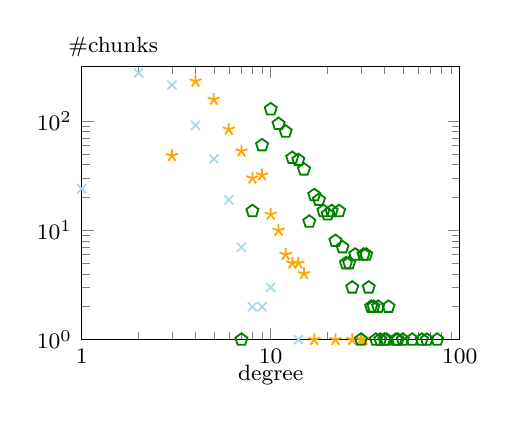
\begin{tikzpicture}[scale=1]
    \begin{axis}[
        height=\columnwidth/2.4,
        width=\columnwidth/1.9,
        ylabel={\#chunks},
        xlabel={degree},
        xmode=log, ymode=log,
        xmin=1, xmax=100,
        ymin=1, ymax=316,
        xtick={1, 10, 100},
        xticklabels={1, 10, 100},
        ytick={1, 10, 100},
        yticklabels={$10^0$, $10^1$, $10^2$},
        every axis y label/.style={at={(current axis.north west)},right=4mm,above=0mm},
        label style={font=\footnotesize},
        tick label style={font=\footnotesize},
        every axis x label/.style={at={(current axis.south)},right=0mm,above=-7mm},
        label style={font=\footnotesize},
        tick label style={font=\footnotesize},
    ]


    \addplot[only marks, mark size=2.3pt, mark=x,color=LightBlue, line width=0.23mm]
        plot coordinates { % SkeTRAG
(1, 24)
(2, 275)
(3, 213)
(4, 91)
(5, 45)
(6, 19)
(7, 7)
(8, 2)
(9, 2)
(10, 3)
(14, 1)
    };

    \addplot[only marks, mark size=2.3pt, mark=star,color=Orange, line width=0.23mm]
        plot coordinates { % SkeTRAG
(3, 48)
(4, 231)
(5, 157)
(6, 84)
(7, 53)
(8, 30)
(9, 32)
(10, 14)
(11, 10)
(12, 6)
(13, 5)
(14, 5)
(15, 4)
(17, 1)
(22, 1)
(27, 1)
(30, 1)
(31, 1)
    };

    \addplot[only marks, mark size=2.3pt, mark=pentagon,color=Green, line width=0.23mm]
        plot coordinates { % SkeTRAG
(7, 1)
(8, 15)
(9, 60)
(10, 128)
(11, 94)
(12, 80)
(13, 46)
(14, 44)
(15, 36)
(16, 12)
(17, 21)
(18, 19)
(19, 15)
(20, 14)
(21, 15)
(22, 8)
(23, 15)
(24, 7)
(25, 5)
(26, 5)
(27, 3)
(28, 6)
(30, 1)
(31, 6)
(32, 6)
(33, 3)
(34, 2)
(35, 2)
(36, 1)
(37, 2)
(38, 1)
(40, 1)
(41, 1)
(42, 2)
(46, 1)
(47, 1)
(50, 1)
(56, 1)
(63, 1)
(67, 1)
(76, 1)
    };

    \end{axis}

\end{tikzpicture}
}%
\hspace{2mm}
\subfloat[$\clen=150$]{
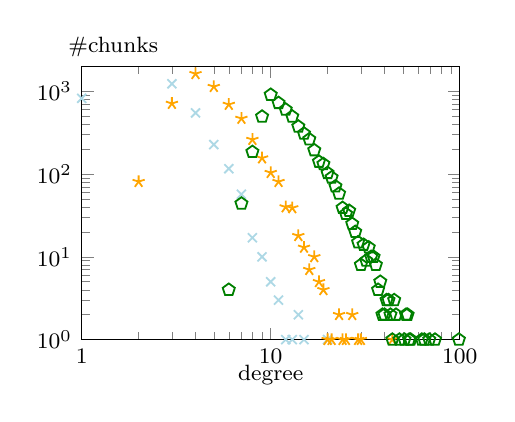
\begin{tikzpicture}[scale=1]
    \begin{axis}[
        height=\columnwidth/2.4,
        width=\columnwidth/1.9,
        ylabel={\#chunks},
        xlabel={degree},
        xmode=log, ymode=log,
        xmin=1, xmax=100,
        ymin=1, ymax=2000,
        xtick={1, 10, 100},
        xticklabels={1, 10, 100},
        ytick={1, 10, 100, 1000},
        yticklabels={$10^0$, $10^1$, $10^2$, $10^3$},
        every axis y label/.style={at={(current axis.north west)},right=4mm,above=0mm},
        label style={font=\footnotesize},
        tick label style={font=\footnotesize},
        every axis x label/.style={at={(current axis.south)},right=0mm,above=-7mm},
        label style={font=\footnotesize},
        tick label style={font=\footnotesize},
    ]


    \addplot[only marks, mark size=2.3pt, mark=x,color=LightBlue, line width=0.23mm]
        plot coordinates { % SkeTRAG
(1, 823)
(2, 2427)
(3, 1230)
(4, 547)
(5, 227)
(6, 116)
(7, 57)
(8, 17)
(9, 10)
(10, 5)
(11, 3)
(12, 1)
(13, 1)
(14, 2)
(15, 1)
(20, 1)
    };

    \addplot[only marks, mark size=2.3pt, mark=star,color=Orange, line width=0.23mm]
        plot coordinates { % SkeTRAG
(2, 81)
(3, 711)
(4, 1628)
(5, 1138)
(6, 692)
(7, 469)
(8, 261)
(9, 156)
(10, 104)
(11, 81)
(12, 40)
(13, 39)
(14, 18)
(15, 13)
(16, 7)
(17, 10)
(18, 5)
(19, 4)
(20, 1)
(21, 1)
(23, 2)
(24, 1)
(25, 1)
(27, 2)
(29, 1)
(30, 1)
(44, 1)
    };

    \addplot[only marks, mark size=2.3pt, mark=pentagon,color=Green, line width=0.23mm]
        plot coordinates { % SkeTRAG
(6, 4)
(7, 44)
(8, 185)
(9, 494)
(10, 907)
(11, 722)
(12, 601)
(13, 495)
(14, 375)
(15, 308)
(16, 263)
(17, 194)
(18, 141)
(19, 132)
(20, 103)
(21, 91)
(22, 71)
(23, 58)
(24, 39)
(25, 33)
(26, 36)
(27, 25)
(28, 20)
(29, 15)
(30, 8)
(31, 14)
(32, 9)
(33, 13)
(34, 10)
(35, 10)
(36, 8)
(37, 4)
(38, 5)
(39, 2)
(40, 2)
(41, 3)
(42, 3)
(43, 2)
(44, 1)
(45, 3)
(46, 2)
(48, 1)
(51, 1)
(52, 2)
(53, 2)
(54, 1)
(55, 1)
(63, 1)
(65, 1)
(69, 1)
(74, 1)
(99, 1)
    };

    \end{axis}

\end{tikzpicture}
}%
\caption{Log-log Plot of the degree distribution of the KNN graph on MuSiQue.}
\label{fig:degree-distribution}
\vspace{-4mm}
\end{figure}

\subsection{Rationale and Comparison}\label{sec:ket-rationale}

\sketrag is motivated by two key observations. First, a small subset of core text chunks often exhibits broad relevance to others. Figure~\ref{fig:degree-distribution} presents the degree distribution of the KNN graph constructed from the MuSiQue dataset with input chunk sizes $\clen = 1200$ and $\clen = 150$. This heavily skewed distribution highlights the importance of core chunks in linking different parts of the graph. Consequently, these core chunks should be prioritized to extract high-quality triplets using the LLM.
Second, in the lightweight alternative graph $\G_k$, keywords and their neighboring text chunks can serve as stand-ins for entities and their ego networks. Specifically, when seed keywords align with seed entities, their neighboring text chunks are expected to contain information about those entities' ego networks. Hence, these neighboring chunks are treated as candidates, and retrieval follows the standard \textrag strategy.

To summarize, compared to previous \kgrag solutions~\cite{li2024dalk,delile2024graph,edge2024local,gutierrez2024hipporag}, \sketrag focuses on a smaller set of core chunks to construct a knowledge graph skeleton while leveraging a text-keyword bipartite graph as a lightweight alternative. This design lowers the cost of LLM inference and improves result quality via two distinct retrieval channels (entity and keyword). Additionally, in the keyword channel, \sketrag confines the retrieval to snippets containing seed keywords, unlike \textrag, which searches across the entire $\Tset$. This subgraph-based approach better captures in-text relationships w.r.t.\ seed keywords, enhancing overall effectiveness.

